\chapter{Convolutional Neural Networks}

\label{chapter:ConvolutionalNeuralNetworks}

% ----------------

\section{Definition}
A Convolutional Neural Network (CNN) is a class of feed-forward neural network. CNN are mainly applied in the fields of computer vision and natural language processing. It has been first presented in \cite{lecun1998gradient}. Recent progresses have led to a gain in interest in this method and also in a broader field called Deep Learning, which is described in \cite{lecun2015deep}. This section is mainly based on this latter article. It has been a great discover because this class of network is able to automatically learn the features to extract from a dataset. Whereas traditionally, the previous works in computer vision were based on hand-engineered features. This difference is essential because the key success factor of CNN is the amount of data and computation power available instead of field knowledge.

CNN are inspired by our visual cortex, in particular, the connectivity pattern between layers of artificial neurons is restricted to a region as it is in our visual system with receptive fields. With this special connectivity pattern, CNN take advantage of natural signals, which are often locally highly correlated. Another property of natural signals is the fact that the local statistics of images are invariant to location. If a motif can appear in one location of an image, it could also appear somewhere else.

CNN are built on top of four key ideas: local connection, shared weights, pooling and use of many layers. The architecture of a typical CNN is composed of these layers; in a first part: convolution layer, ReLU, pooling layer and in a second part: fully connected layer, loss layer.

The convolution layer applies a set of discrete convolutions on the output of the previous layer. Each convolution is done using a kernel (also called: mask, filter bank) and produces a 2D feature map. The feature maps contain high activations if their convolutions have detected an interesting motif. The layer's parameters are the weights in the kernels. This layer can also be seen as a layer with local connections, so that a neuron is only connected to neurons of the previous layer in the same region. Local connections give the ability to the layer to detect local patterns from the previous layer. Moreover, the weights of the local connections are shared among all neurons in the layer, this means that the same local pattern can be detected in the same way anywhere in the previous layer.

\begin{figure*}
	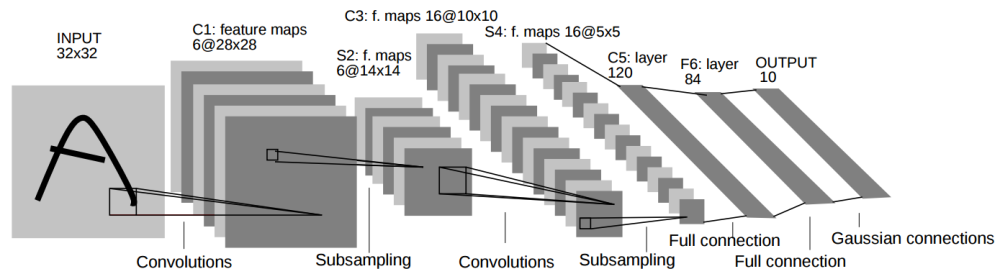
\includegraphics[width=\textwidth]{img/cnn.png}
	\caption{Architecture of LeNet-5, a basic Convolutional Neural Network}
	\label{fig:cnn}
\end{figure*}

The ReLU (Rectified Linear Units) applies a non-linear function $f(x) = \max(0, x)$ to the output of the previous convolution layer. Other non-linear activation function are available: hyperbolic tangent or sigmoid function for example. The ReLU is the most common because the training of the neural network is faster with it \cite{krizhevsky2012imagenet}.

The pooling layer splits the output of the previous layer into a grid, then on each cell of the grid a pooling function is applied and outputs only a single value. Thus, the pooling layer is a down-sampling step, the resolution of the grid can vary and affects the sampling rate. This layer merges multiple semantically similar features into one. Due to the down-sampling, the position of the feature is not accurately preserved, therefore an invariance to small shifts or distortions is spawned. In fact, the position of a feature is not as important as its relative position to others features. A typical pooling function outputs the maximum value of a local patch.

Repeating these layers several times in this order: convolution, ReLU, pooling, one can exploit the fact that high level features are composed of lower level features. The first group of layers can detect small details such as edges and contours. The second layer can detect higher level features such as motifs, and so on. This process is repeated so that firstly, edges are merged into motifs, motifs into parts and finally parts into objects. The architecture of a very basic CNN is shown in figure \ref{fig:cnn}.

After this first part composed of convolution layers, ReLU, pooling layers, a second part of the neural network is composed of fully-connected layers and a loss layer. This second part is a classical feed-forward neural network used to classify the features coming from the first part. The training of CNN is possible using the backpropagation algorithm. Because of the local connectivity and the shared weights, there is less parameters in the model thus the network is less prone to overfitting and generalizes better.

\section{Usage}
Convolutional neural networks are mostly used in supervised learning for classification tasks. One of the first successful commercial application was to recognise handwritten digits on bank checks \cite{lecun1998gradient}. In this task, the system is given a normalized, grayscale, 28-by-28 pixels image of a digit and outputs the class of the image: zero, one, two, and so on until nine. The same technique can be used for Optical Character Recognition (OCR). By using a sliding window on an image, it is possible to use a CNN to recognize if a face is depicted at a certain position \cite{garcia2004convolutional}. It is possible to use CNN for image classification \cite{krizhevsky2012imagenet}, for example the ImageNet dataset is composed of roughly 1.2 million images divided into 1,000 classes, the goal being to predict the class of a given image. Scene labeling consists in labeling each pixel in an image with the category of the object it belongs to. CNN have been successfully applied to this task \cite{farabet2013learning}. It is useful for example to self-driving cars and more generally to autonomous robots. When used with one dimensional convolution, CNN are able to process acoustic signals for automatic speech recognition \cite{sercu2015verydeep}.

\section{Feature extraction}
Recent work showed that the representation learned by the CNN is a good descriptor for image retrieval. With the AlexNet network \cite{krizhevsky2012imagenet}, one can use the feature activations induced by an image at the last hidden layer to represent an image. Experiments has shown that semantically similar images get a similar feature vector in a Euclidean space, even if the images are not close in L2. The only drawback is that the representation is a real-valued vector of dimension 4096. Therefore, the computation of the distance between two vectors is expensive, moreover the storage cost could also be an issue. To tackle this issue, the authors suggest a dimensionality reduction with an auto encoder.

In a later paper \cite{babenko2014neural}, the performance of feature vectors extracted with CNN in the context of image retrieval is studied more in depth. The conclusion is that CNN performs well for image retrieval, even if the network is trained on an unrelated classification task. The performances can be improved with a fine tuning on a dataset similar to the retrieval dataset. For example, by using a neural network trained on ImageNet to retrieve landscape images, the performances are good. Unsurprisingly, after a retraining on a dataset composed of landscape images the performances become even better. The compression with PCA is also investigated, and the retrieval performance is not too much affected when compared to other state of the art descriptors. Image features extraction with CNN, for all these reasons, seems to be very promising for image retrieval.

\section{Models}
\label{chapter:ConvolutionalNeuralNetworks:section:Models}
In this section, three models used for the ImageNet Large Scale Visual Recognition Challenge (ILSVRC) are presented. All of them are implemented in the Keras \cite{chollet2015keras} library and are used later in this thesis.

The VGG network \cite{simonyan2014verydeep} was created in 2014 for ILSVRC. The authors investigated the effect of depth on the accuracy. For that purpose, they use a simple convolutional neural network with very small (3x3) convolution filters with stride and pad of 1, 2x2 maxpooling with stride 2, and push the depth to 16-19 layers, which was a lot at the time. VGG16 and VGG19 are detailed in table \ref{table:vgg_model}.

\begin{table}[h]
\centering
\caption{Configurations of VGG16 and VGG19 networks. The convolutional layer parameters are denoted as "`conv(receptive field size)-(number of channels)"'. The ReLU activation is not shown for brevity.}
\label{table:vgg_model}
\begin{tabular}{|c|c|}
\hline
VGG16                     & VGG19                     \\
\hline
\multicolumn{2}{|c|}{input (224x224 RBG image)}       \\
\hline
conv3-64                  & conv3-64                  \\
conv3-64                  & conv3-64                  \\
\hline
\multicolumn{2}{|c|}{maxpool}                         \\
\hline
conv3-128                 & conv3-128                 \\
conv3-128                 & conv3-128                 \\
\hline
\multicolumn{2}{|c|}{maxpool}                         \\
\hline
conv3-256                 & conv3-256                 \\
conv3-256                 & conv3-256                 \\
\textbf{conv3-256}        & conv3-256                 \\
                          & \textbf{conv3-256}        \\
\hline
\multicolumn{2}{|c|}{maxpool}                         \\
\hline
conv3-512                 & conv3-512                 \\
conv3-512                 & conv3-512                 \\
\textbf{conv3-512}        & conv3-512                 \\
                          & \textbf{conv3-512}        \\
\hline
\multicolumn{2}{|c|}{maxpool}                         \\
\hline
conv3-512                 & conv3-512                 \\
conv3-512                 & conv3-512                 \\
\textbf{conv3-512}        & conv3-512                 \\
                          & \textbf{conv3-512}        \\
\hline
\multicolumn{2}{|c|}{maxpool}                         \\
\hline
\multicolumn{2}{|c|}{FC-4096}                         \\
\hline
\multicolumn{2}{|c|}{FC-4096}                         \\
\hline
\multicolumn{2}{|c|}{FC-1000}                         \\
\hline
\multicolumn{2}{|c|}{soft-max}                        \\
\hline
\end{tabular}
\end{table}

The InceptionV3 network \cite{szegedy2015rethinking} was created in 2015. Instead of stacking convolutional and pooling layers sequentially on top of each others, some layers are in parallel and their results are merged periodically. As shown in figure \ref{fig:inceptionv3} from Google Research Blog \footnote{https://research.googleblog.com/2016/03/train-your-own-image-classifier-with.html}, the key idea of this network is to stack Inception modules, which are composed of convolutional and pooling layers. This can be easily seen in figure \ref{fig:inceptionv3}. By using fewer weights than previous neural networks, for instance about 30x fewer parameters than VGG19, the computational cost of InceptionV3 is suitable for big-data or mobile scenarios.

\begin{figure}[h]
	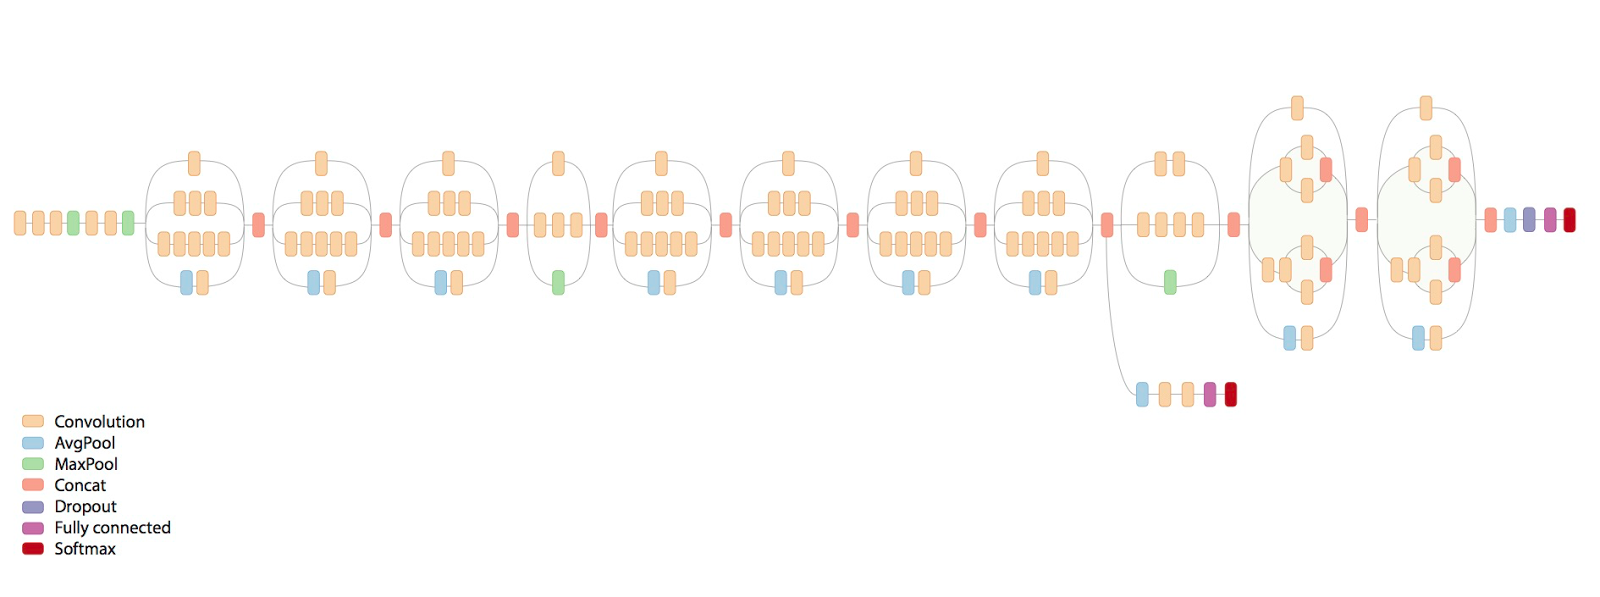
\includegraphics[width=\textwidth]{img/inceptionv3.png}
	\caption{Architecture of the InceptionV3 network.}
	\label{fig:inceptionv3}
\end{figure}

The ResNet50 network \cite{kaiming2015deepresidual} was created in 2015 for ILSVRC. The authors use a 50 layers Residual Network, whose key idea is to introduce shortcuts connections into a sequential network. As networks are becoming deeper, the learning is more difficult because of the vanishing/exploding gradient problem. In particular, with the network depth increasing, accuracy gets saturated and then degrades rapidly. The idea behind shortcuts in Residual Networks is to by-pass a set of layers if they are not useful to improve the accuracy of the whole network. Thus, in theory, it is possible to stack as many building blocks as possible without affecting the accuracy, because unnecessary blocks can be skipped. Figure \ref{fig:renet50} shows a Residual Network with 34 layers

\begin{figure}[p]
	\centering
	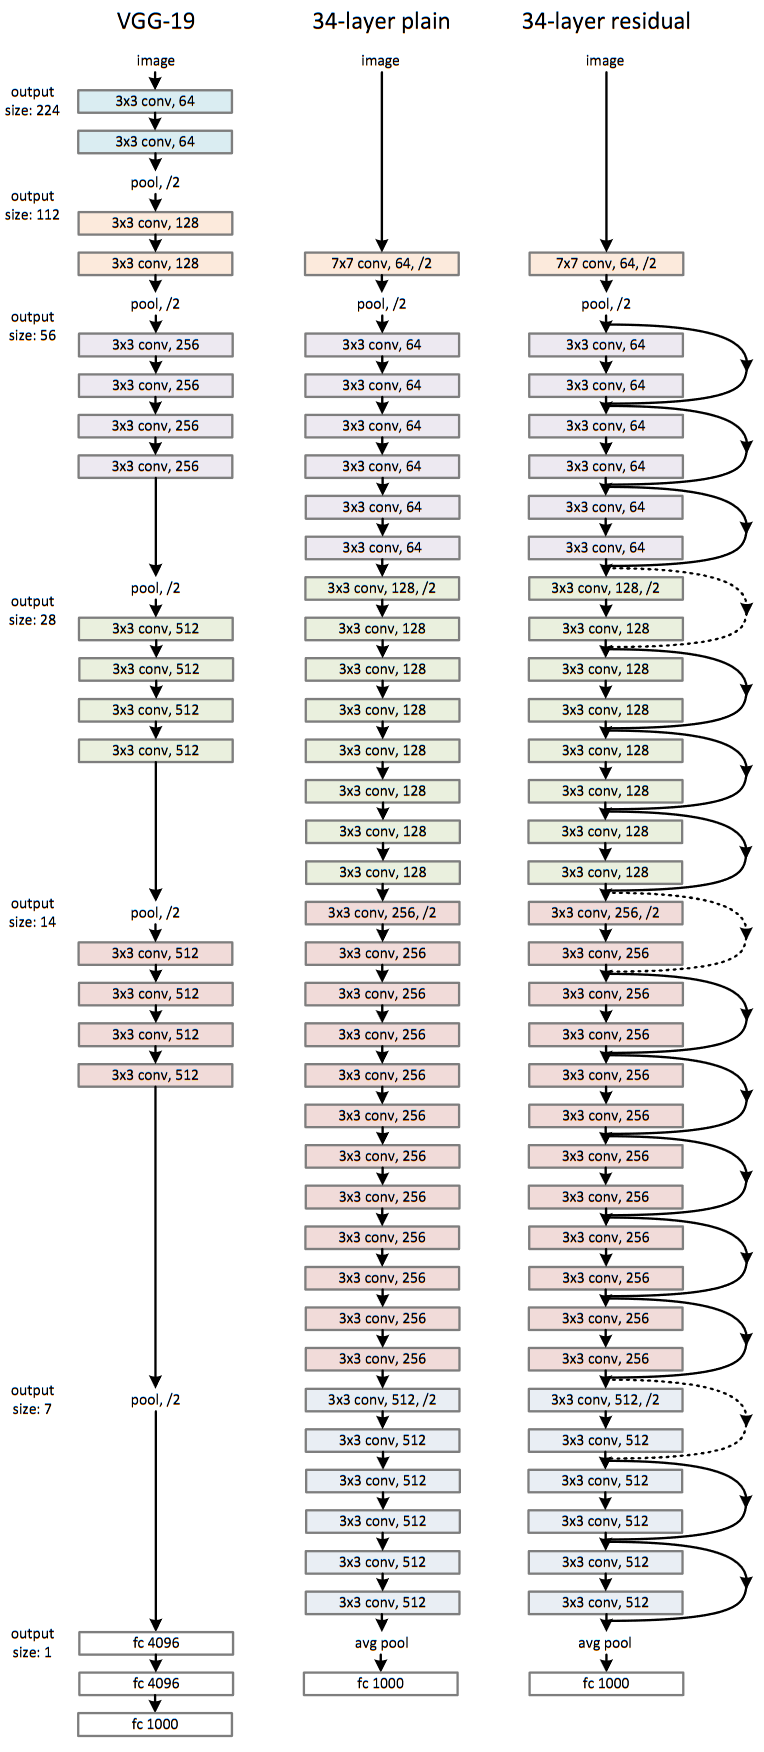
\includegraphics[height=0.9\textheight]{img/resnet34.png}
	\caption{\textbf{Left}: the VGG19 model as a reference. \textbf{Middle}: a plain network with 34 parameters layers. \textbf{Right}: a Residual Network with 34 parameter layers. The dotted shorcuts increase dimensions.}
	\label{fig:renet50}
\end{figure}
